\documentclass[tikz,border=2pt]{standalone}
\usepackage{amsmath}
\usetikzlibrary{arrows.meta}
\begin{document}
% Deferred whole life insurance, u = 5: no benefit for death in [0,5]; after 5 a unit benefit is paid at death.
% Valued at age x+5 the cover is bar A_{x+5} = 0.4; multiplying by {}_5E_x = 0.7 gives 0.28 at issue.
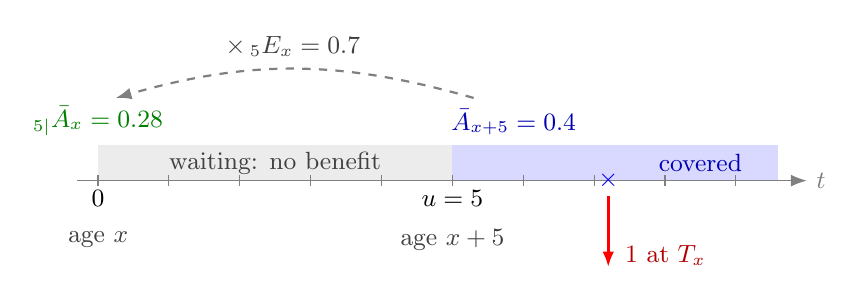
\begin{tikzpicture}[font=\small, >={Latex[length=2mm]}, x=0.9cm, y=1cm]
  \fill[gray!15] (0,0) rectangle (5,0.45);
  \fill[blue!15] (5,0) rectangle (9.6,0.45);
  \draw[gray, ->] (-0.3,0) -- (10,0) node[right] {$t$};
  \foreach \k in {0,...,9} \draw[gray] (\k,-0.07) -- (\k,0.07);
  \node[below, inner sep=2pt] at (0,-0.05) {$0$};
  \node[below, inner sep=2pt] at (5,-0.05) {$u=5$};
  \node[gray!50!black] at (0,-0.75) {age $x$};
  \node[gray!50!black] at (5,-0.75) {age $x+5$};
  \node[gray!50!black] at (2.5,0.225) {waiting: no benefit};
  \node[blue!70!black] at (8.5,0.225) {covered};
  % death after the waiting period
  \node[blue] at (7.2,0) {$\times$};
  \draw[->, red, very thick] (7.2,-0.2) -- (7.2,-1.1);
  \node[red!70!black, anchor=west] at (7.3,-0.95) {$1$ at $T_x$};
  % value of the cover at age x+5, brought back to issue
  \node[blue!70!black, anchor=south west, inner sep=2pt] at (4.9,0.5) {$\bar A_{x+5}=0.4$};
  \draw[->, gray, thick, dashed] (5.3,1.05) to[bend right=16] (0.25,1.05);
  \node[gray!50!black, anchor=south] at (2.75,1.45) {$\times\,{}_5E_x=0.7$};
  \node[green!50!black, anchor=south, inner sep=2pt] at (0,0.5) {${}_{5|}\bar A_x=0.28$};
\end{tikzpicture}
\end{document}
